\clearpage
\subsection{Definition of \texorpdfstring{\alphat}{AlphaT}\label{sec:alphat}}

Multi-jet events stemming from QCD contribute overwhelmingly to
all-hadronic events recorded by the detector. Generally, these QCD events
have no significant inbalance in transverse energy and can 
be reduced with a requirement for high-\met. Yet, this approach has proven difficult, 
as the calculation of \met is sensitive to detector effects and conditions, 
and additionaly, in the high-\met phase space systematic uncertainties become difficult
to control. The variable, \alphat, introduced in 2008 by Randall and 
Tucker-Smith~\cite{Randall:2008rw} effectively supresses multi-jet 
events with no significant met without relying on the measurment
of \met. By construction it also introduces robustness against mismeasurements 
of transverse eneriges in multi-jet systems.  In the simplest case of a two-jet system,
\alphat is defined as
\begin{equation}
\label{eq:alphat}
\alphat\, =\, \frac{\Et^{{\rm j}_2}}{M_\text{T}} \, ,
\end{equation}

where $\Et^{\rm j_2}$ is the transverse energy of the less energetic
jet and $M_\text{T}$ is the transverse mass of the dijet system,
defined as

\begin{equation}
  \label{eq:mt}
  M_\text{T}\, = \,\sqrt{ \left( \sum_{i=1}^2 \Et^{{\rm j}_i}
    \right)^2 - \left( \sum_{i=1}^2 p_x^{{\rm j}_i} \right)^2 - \left(
      \sum_{i=1}^2 p_y^{{\rm j}_i} \right)^2} \, = \,\sqrt{\scalht^2 + \left(\mht\right)^2} \,  .
\end{equation}

where $\Et^{{\rm j}_i}$, $p_x^{{\rm j}_i}$, and $p_y^{{\rm j}_i}$ are,
respectively, the transverse energy and $x$ or $y$ components of the
transverse momentum of jet ${\rm j}_i$. In well measured QCD dijet events, 
transverse momentum conservation requires the $\pT$ of the two jets to be 
of equal magnitude and back-to-back in the plane transverse to the beam.
The value of \alphat for these type of events can be best seen
after transforming equation~\ref{eq:mt} into CMS coordinates:

\begin{equation}
  \label{eq:mt-polar}
  \alphat\, = \,\frac{\Et^{{\rm j}_2}}{\sqrt{2\Et^{{\rm j}_1}
   \Et^{{\rm j}_2} \left(1-cos\left(\Delta\phi\right)\right)}}\, .
\end{equation}

Well balanced back-to-back jets have \alphat values of 0.5 
For the case of an imbalance in the measured transverse energies 
of back-to-back jets \alphat is reduced to values smaller than 0.5, 
this gives the variable its robustness with respect to jet energy 
mismeasurements. Figure~\ref{fig:alphat_dist} shows the \alphat 
distribution in two jet multiplicity bins for events passing 
an HT trigger and basic pre-selection requirments. Multi-jet 
events from QCD drop to neglible levels above $\alphat>$ 0.55
while events with genuine \met continue to populate bins in excess
of  $\alphat>$ 0.55.

In the case where the two 
jets are not back-to-back in the transverse plane but rather the 
dijet system balances genuine \met, for example in leptonically 
decaying W boson recoiling off a syetem of jets, the values of 
\alphat can exceed 0.5.

\begin{figure}[h!t]
  \begin{center}
    \subfigure[\label{fig:alphat_le3j}]{
      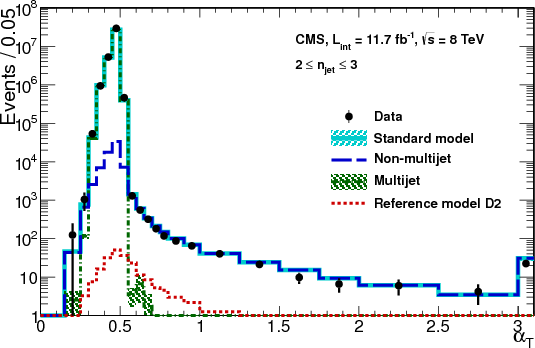
\includegraphics[width=0.45\textwidth,]{figures/data-mc/AlphaT_le3j.png}
    } 
    \subfigure[\label{fig:alphat_ge4j}]{
      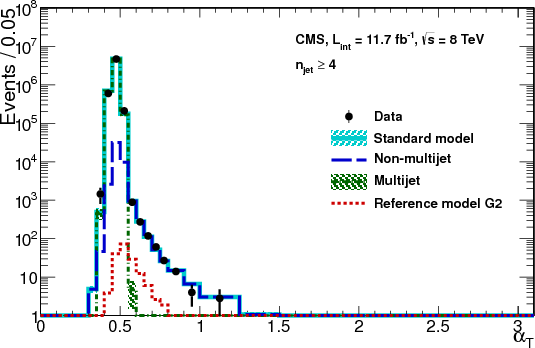
\includegraphics[width=0.45\textwidth,]{figures/data-mc/AlphaT_ge4j.png}
    } \\
    \caption{\alphat distribution from~\cite{RA1Paper2012} }
    \label{fig:alphat_dist}
  \end{center}
\end{figure}

An extension of \alphat calculation can be made for systems of 
more than two jets~\cite{cms-pas-sus-09001} by clustering the jets into a 
two pseudo-jets system. A pseudo-jet's $\Et$ is calculated
as the scalar sum of the contributing jets' transverse energy, while the total
transverse energy of the system, \scalht, is defined as the scalar sum of the 
pseudo-jet's transverse energy: $\scalht = \Et^{{\rm pj}_1}+\Et^{{\rm pj}_2}$.
All combinations of the n-jet system are tested, and the configuration which
balances the constructed pseudo-jets' \Et is chosen, ie the combinations which
minimized $\dht = \Et^{{\rm pj}_1}-\Et^{{\rm pj}_2}$. As balanced QCD events
are expected to have small \dht, this simple clustering criterion provides the best
separation between QCD events and events with genuine \met. 
Equation~(\ref{eq:alphat}) can therefore be generalised as:

\begin{equation}
  \label{eq:alphat2}
  \alphat\, = \,\frac{1}{2} \times \frac{\scalht -
    \dht}{\sqrt{\scalht^2 - \mht^2}} \, = \,\frac{1}{2} \times 
  \frac{1 - (\dht/\scalht)}{\sqrt{1 - (\mht/\scalht)^2}} \, . 
\end{equation}

In the limit that  $\dht \rightarrow 0$, the ratio of missing energy and
visible energy can be expressed as a function of \alphat:

\begin{equation}
  \label{eq:alphat3}
  \frac{\mht}{\scalht} \, = \, \sqrt{ 1 - \frac{1}{4 \cdot \alphat^2} }
\end{equation}

This analysis uses an \alphat threshold of 0.55, which results in events
having more than 40\% percent as much missing transverse energy as visible transverse
energy. For an event with $\scalht=$~375~\gev, this amounts to nearly 160 GeV in \mht.  
%For reference, under the assumption of $\dht = 0$, the values of
%$\alphat = 0.55$, 0.60, and 0.65 map onto values of the ratio
%$\mht/\scalht = 0.42$, 0.55, and 0.64.
%
